\documentclass{article}
\usepackage[utf8]{inputenc}
\usepackage[spanish]{babel}
\usepackage{listings}
\usepackage{graphicx}
\usepackage{hyperref}
\graphicspath{ {images/} }
\usepackage{cite}

\begin{document}

\begin{titlepage}
    \begin{center}
        \vspace*{1cm}
            
        \Huge
        \textbf{Parcial 1}
            
        \vspace{0.5cm}
        \LARGE
        Informática II
            
        \vspace{2.5cm}
            
        \textbf{Alejandra Calle Vasquez\\
                Jesús David Mercado Machado \\
                Juan Sebastian Garavito Gallo}
            
        \vfill
            
        \vspace{0.7cm}
            
        \Large
        Despartamento de Ingeniería Electrónica y Telecomunicaciones\\
        Universidad de Antioquia\\
        Medellín\\
        Abril de 2021
            
    \end{center}
\end{titlepage}

\tableofcontents
\newpage
\section{Analisis del problema}\label{intro}
\textbf{Organización de los leds: }
Para la optimización de la conexión y organización de los leds usamos 8 integrados 74HC595 los cuales nos permiten formar un sistema de ubicación de cada bombillo, a cada uno de estos integrados le asignamos 8 leds; que sería lo máximo que podríamos controlar por cada uno de ellos, de este modo formariamos la matriz 8x8 que se es requerida para realizar el ejercicio. Esta manera de conexión de los leds nos pareció optima por que solo conlleva al uso de tres pines.

\section{Circuito inicial en Tinkercad} \label{imagenes}

\begin{figure}[h]
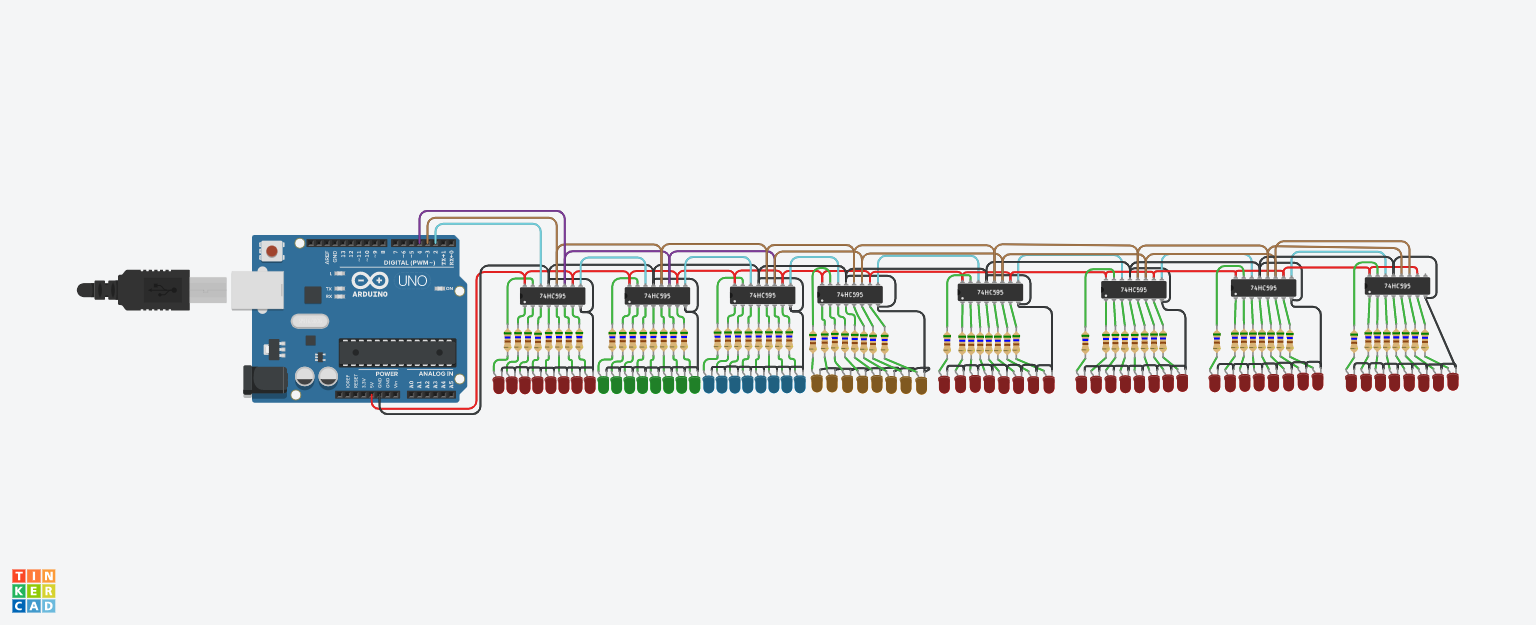
\includegraphics[width=15cm]{PARCIAL INFO 2.png}
\centering
\caption{Primeras conexiones}
\label{fig:PARCIAL INFO 2}
\end{figure}
\newpage

\subsection{Patron determinado}
\textbf{Organización matricial de los leds (Para verificar funcionamiento): }
En este caso organizamos nuestros leds de modo que se pueda ver el tablero en forma de matriz y usamos unos patrones establecidos para corroborar su funcionamiento. 
 
\begin{figure}[h]
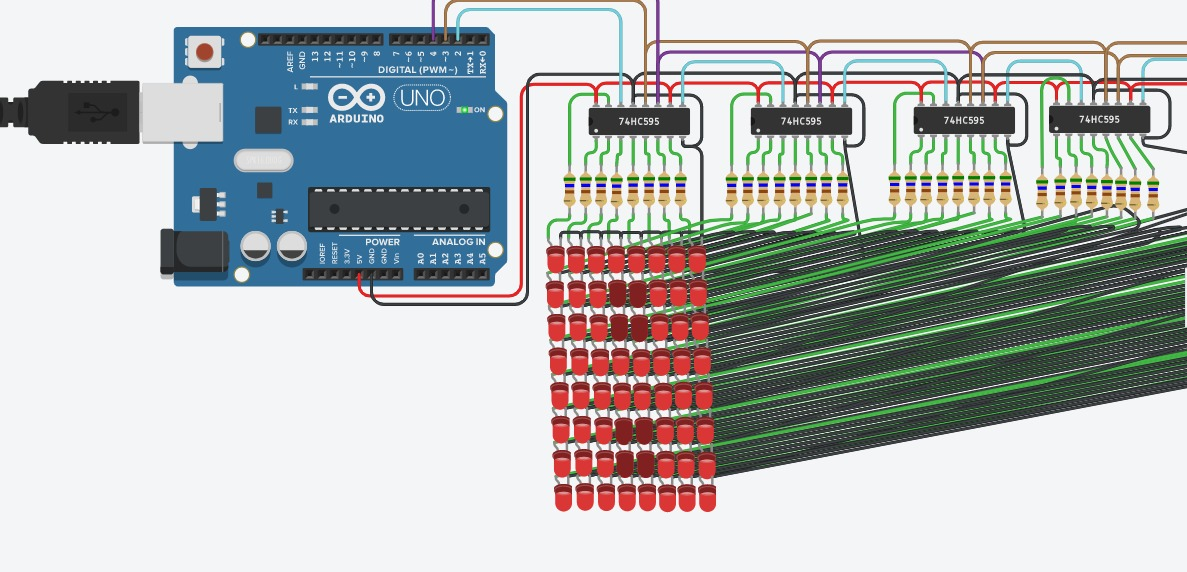
\includegraphics[width=7cm]{imagen2.jpeg}
\caption{Simulación del tablero, signo C}
\label{fig:imagen2}
\end{figure}

\begin{figure}[h]
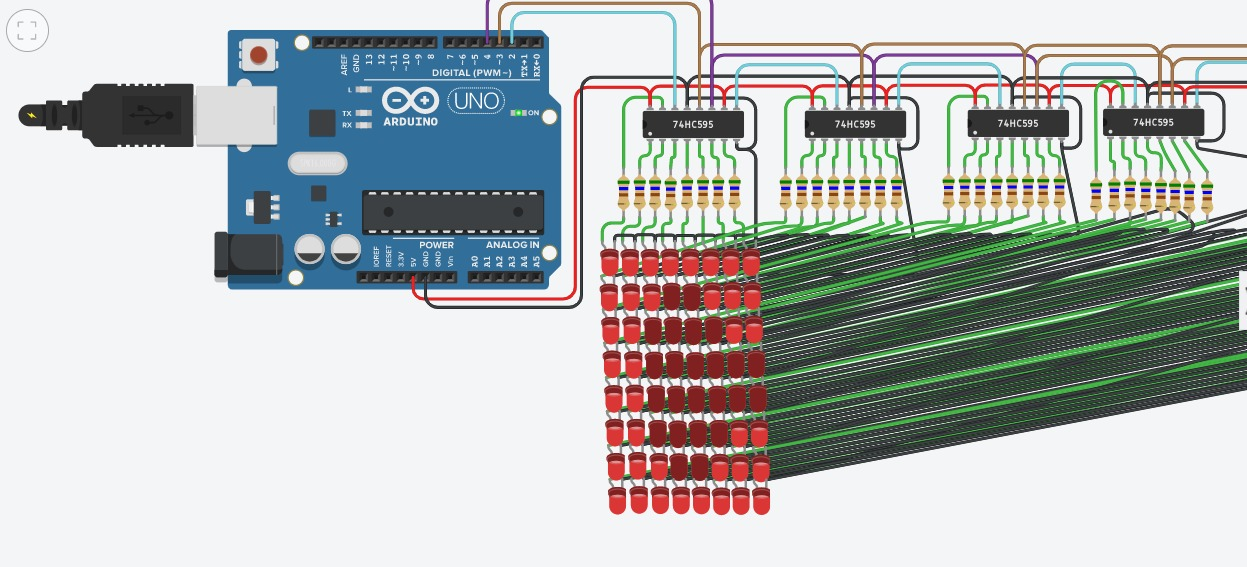
\includegraphics[width=7cm]{imagen3.jpeg}
\caption{Simulación del tablero, signo B}
\label{fig:imagen3}
\end{figure}


\subsection{Interpretación del patron predeterminado}
Para representar estos codigos predeterminados usaremos entradas de 1 y 0 para representar los patrones con las siguientes clasificaciones
\textbf{1=Endendido}
\textbf{0=Apagado}

\vspace{0.7cm}
\begin{figure}[h]
\centering
\subfloat [Tablero signo C]
\label{fig:imagenC}
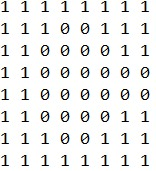
\includegraphics[width=3cm]{imagenC.jpeg}
\subfloat [Tablero signo B]
\label{fig:imagenB}
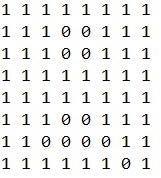
\includegraphics[width=3cm]{imagenB.jpeg}
\end{figure}

\newpage

\section{Algoritmo implementado} \label{codigo}
\textbf{Main principal}

\ref{avancecodigo.ino}
\begin{lstlisting}[language=C++, label=avancecodigo.ino]

int incomingByte = 0; // for incoming serial data
int aux=0;
int cont=0;
void setup() {
  Serial.begin(9600); // opens serial port, sets data rate to 9600 bps
}

void loop() {
  // send data only when you receive data:
  if (Serial.available() > 0) {
    // read the incoming byte:
    if(cont<9)
    {
      aux=Serial.read();
      incomingByte+=(aux-48)*pow(2,cont-1);
    }

    else
    {
    	Serial.print("I received: ");
    	Serial.println(incomingByte);
      	cont=0;
    }
    cont++;
  }
}

 \end{lstlisting}
 
 
\subsection{implementación}
Lo que tratamos de lograr con el código anteriormente presentado es pedir fila por fila al usuario lo que quiere representar en el tablero de leds, de esta manera estaremos recibiendo los datos en ascii para luego pasarlos a  binario y así llegar a los tableros con las entradas en unos y ceros (como se ve representado en el punto 2.2), pero al momento de hacer la conversión nos quedaría un solo valor, esto significa que si el usuario ingresa una fila entera de "1" solo tendríamos que almacenar el valor 255; que es el equivalente, para luego imprimirlo.





\newpage
\subsection{Código que llevamos elaborado hasta el momento}
date: 21/04/2021
\begin{lstlisting}[language=C++, label=codigocompleto]

char digito='0';
int cont=7,columna=0,*matriz;
int pinData  = 2;
int pinLatch = 3;
int pinClock = 4;
void setup() {
  Serial.begin(9600);
  pinMode(pinData, OUTPUT);
  pinMode(pinLatch, OUTPUT);
  pinMode(pinClock, OUTPUT);
}
int* Lectura() {
   // send data only when you receive data:
  	int incomingByte[8];
  	for(int i=0;i<8;i++)
  	{
    	incomingByte[i]=0;
  	}

    while(Serial.available() > 0)
    {
      digito=Serial.read();
      Serial.println(digito); 
      Serial.println(columna);
      if(digito=='1')
          {
            incomingByte[columna]+=(pow(2,cont)+0.5);
        	cont--;
          }
      else if(digito=='0')
      {
        cont--;
      }
      if(cont==-1){
        Serial.println(incomingByte[columna]);
        Serial.print("Ahora ingrese la siguiente fila de matrix:");
        Serial.println(columna+1);
        cont=7;
        columna++;
      }
      if(columna==7)
      {
        return incomingByte;
      }
    }
}
void ledWrite(int matriz[8]){
   for(int i=0;i<8;i++)
   {   
    	shiftOut(pinData, pinClock, LSBFIRST, *(matriz+i));
   }
  		digitalWrite(pinLatch, HIGH);
   		digitalWrite(pinLatch, LOW);
}

void loop()
{
  matriz=Lectura();
  ledWrite(matriz);
  
}
 \end{lstlisting}
 
\textbf{Hasta este punto del código tenemos completa la recepción de datos.}



\vspace{0.5cm}
\subsection{Actualización del código}
date: 22/04/2021
\begin{lstlisting}[language=C++, label=codigocompleto2]

char digito='0';
unsigned short int cont=7,columna=0,pinData  = 2,pinLatch = 3, pinClock = 4;
int *matriz,aux[8];
void setup() {
  Serial.begin(9600);
  pinMode(pinData, OUTPUT);
  pinMode(pinLatch, OUTPUT);
  pinMode(pinClock, OUTPUT);
  for(int i=0;i<8;i++)
      {
        aux[i]=0;
      }

  //matriz=Lectura(aux);
}
int Lectura(int incomingByte[8]) {
   // send data only when you receive data:}
    while(Serial.available() > 0)
    {
      digito=Serial.read();
      //Serial.print("Digito a evaluar:");
      //Serial.println(digito); 
      //Serial.print("Sumatoria:");
      //Serial.println(incomingByte[columna]);
      if(digito=='1')
          {
            incomingByte[columna]+=(pow(2,cont)+0.5);
          cont--;
          }
      else if(digito=='0')
      {
        cont--;
      }
      if(cont==-1){
        //Serial.print("Valor a ingresar:");
        Serial.println(incomingByte[columna]);
        //Serial.print("Ahora ingrese la siguiente fila de matrix:");
        //Serial.println(columna+2);
        cont=7;
        columna++;
      }
    }
  return columna;
}
void ledWrite(int matriz[8]){
   for(int i=0;i<8;i++)
   {   
      shiftOut(pinData, pinClock, LSBFIRST, matriz[i]);
   }
      digitalWrite(pinLatch, HIGH);
      digitalWrite(pinLatch, LOW);
}

void loop()
{
  for(int e=0;e<8;e++)
  {
    Lectura(aux);
  }
  ledWrite(aux);
}

 \end{lstlisting}
 
\textbf{Este código tiene la capacidad de recibir el patrón ingresado por el usuario y los introduce en el tablero de leds.}
 
 
 
 
 
 

\subsection{Actualización del código}
\textbf{-Código final: función de verificación.}

date: 22/04/2021
\begin{lstlisting}[language=C++, label=codigocompleto2]
 
 char digito='0',digito1='0';
unsigned short int cont=7,colo=0,columna=0,pinData  = 2,pinLatch = 3, pinClock = 4;
int aux[8];
bool ciclo = true;
void setup() {
  Serial.begin(9600);
  pinMode(pinData, OUTPUT);
  pinMode(pinLatch, OUTPUT);
  pinMode(pinClock, OUTPUT);
  Serial.println("Desea verificar los leds?introduzca v");
  Serial.println("Desea introducir un patron? indtroduzca i");
  for(int i=0;i<8;i++)
      {
        aux[i]=0;
      }
}
void imagen()
{
  if(Serial.available()>0)
	{
       for(int i=0;i<8;i++)
       {
         colo=Lectura(aux);
       }
    }
  if(colo==8)
  {
    ledWrite(aux);
  }
}
void verificacion()
{
  for(int i=7;i>-1;i--)
   {   
      shiftOut(pinData, pinClock, LSBFIRST, 255);
   }
      digitalWrite(pinLatch, HIGH);
      digitalWrite(pinLatch, LOW);
}
int Lectura(int incomingByte[8]) {
    while(Serial.available() > 0)
    {
      digito=Serial.read();
      if(digito=='1')
          {
            incomingByte[columna]+=(pow(2,cont)+0.5);
          cont--;
          }
      else if(digito=='0')
      {
        cont--;
      }
      if(cont==-1){
        Serial.println(incomingByte[columna]);
        cont=7;
        columna++;
      }
    }
  return columna;
}
void ledWrite(int matriz[8]){
   for(int i=7;i>-1;i--)
   {   
      shiftOut(pinData, pinClock, LSBFIRST, matriz[i]);
   }
      digitalWrite(pinLatch, HIGH);
      digitalWrite(pinLatch, LOW);
}

void loop()
{
  digito1=Serial.read();
  if(digito1=='i')
  {
    Serial.println("Introduzca el patron:");
    while(ciclo==true)imagen();
  }
  if(digito1=='v')verificacion();
}
 
 
 
\end{lstlisting} 



\newpage

\section{Problemas de desarrollo} \label{codigo}

\begin{lstlisting}[language=C++, label=avancecodigo]
char digito='0';
int incomingByte=0;
void setup() {
  Serial.begin(9600); // opens serial port, sets data rate to 9600 bps
}

void loop() {
   // send data only when you receive data:
    while(Serial.available() > 0)
    {
    	for(int cont=0;cont<8;cont++)
    	{
      	  digito=Serial.read();
          if(digito=='1')
          {
            //Serial.print("contador:");
            //Serial.println(cont);
            incomingByte+=pow(2,cont)+0.5;
            //Serial.print("potencia:");
            //Serial.println(pow(2,cont)+0.5);
            Serial.print("Sumatoria:");
            Serial.println(incomingByte);
          }
        }
  	}
}
 \end{lstlisting}

\textbf{1er error: } En las lineas 151 y 154 de esta parte del código tenemos dos comentarios que hacen que el código se dañe, lo que no nos parece lógico ya que los comentarios no deberían afectar en nada. 
 
\textbf{2do error: } El 0.5 que pusimos en en el <pow> es por que <pow> retorna un flotante y que si lo conviertes al entero no dal el resultado en tipo entero si no un numero menor. 

\textbf{3er error: } En el punto 3.4 del trabajo presentamos nuestro código final, en el cual tenemos que aclarar que no guarda los patrones, solo los imprime de a uno y hay que volver a preguntar de nuevo al usuario si quiere ingresar uno nuevo.

\newpage
\section{Link del trabajo en Tinkercad e imágen final} \label{codigo}
\begin{figure}[h]
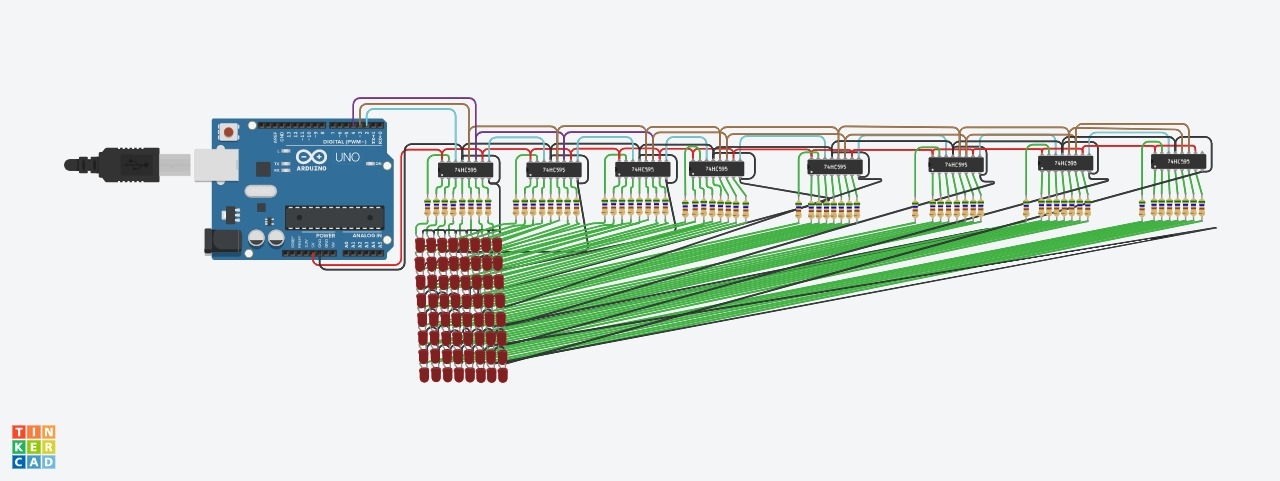
\includegraphics[width=15cm]{Final.jpeg}
\centering
\caption{Primeras conexiones}
\label{fig:Final.jpeg}
\end{figure}

\url{https://www.tinkercad.com/things/4hfqVzkZiJp-copy-of-parcial-info-2/editel?sharecode=RTV-Vb53Aah1mQWeqY-uc4S1DDYA2368JWZUj1CbHhc}





\end{document}